\documentclass[tikz, border=10pt]{standalone}
\usepackage{amsmath}
\usepackage{tikz}
\usetikzlibrary{decorations.pathmorphing, arrows.meta, calc, backgrounds}

\definecolor{navybg}{RGB}{13,27,42}
\definecolor{source1col}{RGB}{0,220,255}
\definecolor{source2col}{RGB}{255,165,0}
\definecolor{photoncol}{RGB}{255,215,0}
\definecolor{starglow}{RGB}{255,255,200}
\definecolor{labelcol}{RGB}{220,220,220}
\definecolor{plotbg}{RGB}{25,40,60}
\definecolor{axiscol}{RGB}{180,180,180}
\definecolor{histcol}{RGB}{100,180,255}

\begin{document}
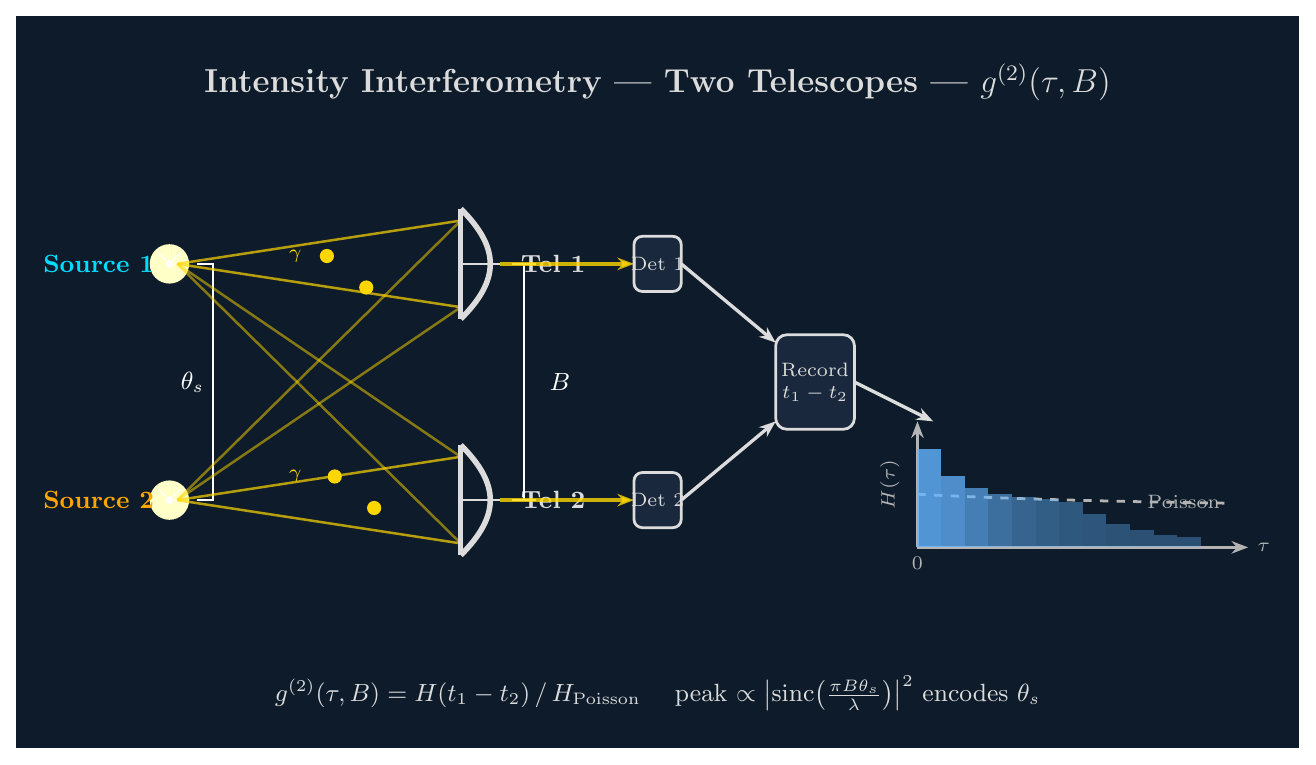
\begin{tikzpicture}[
    background rectangle/.style={fill=navybg},
    show background rectangle,
    arr/.style={-{Stealth[length=6pt]}, line width=1.2pt},
    arrthin/.style={-{Stealth[length=4pt]}, line width=0.8pt},
    mybox/.style={draw=labelcol, fill=plotbg, rounded corners=4pt,
                  line width=1pt, text=labelcol, font=\small,
                  inner sep=5pt, align=center},
]

\path[use as bounding box] (0,0) rectangle (16,9);

% ════════════════════════════════════════════════════════
% 0. TITLE
% ════════════════════════════════════════════════════════
\node[text=labelcol, font=\large\bfseries] at (8.0, 8.3)
    {Intensity Interferometry \textemdash\ Two Telescopes
     \textemdash\ $g^{(2)}(\tau, B)$};

% ════════════════════════════════════════════════════════
% 1. TWO POINT SOURCES (LEFT)
% ════════════════════════════════════════════════════════
\coordinate (S1) at (1.8, 6.0);
\coordinate (S2) at (1.8, 3.0);

\foreach \r/\op in {0.25/15, 0.15/30, 0.08/60}{
    \fill[starglow, opacity=\op] (S1) circle (\r);
}
\fill[white] (S1) circle (0.05);
\foreach \ang in {0,45,90,135}{
    \draw[white, line width=0.6pt, opacity=0.8]
        ($(S1)+(\ang:0.06)$) -- ($(S1)+(\ang:0.20)$);
}
\node[text=source1col, font=\small\bfseries, left=2pt] at (S1) {Source 1};

\foreach \r/\op in {0.25/15, 0.15/30, 0.08/60}{
    \fill[starglow, opacity=\op] (S2) circle (\r);
}
\fill[white] (S2) circle (0.05);
\foreach \ang in {0,45,90,135}{
    \draw[white, line width=0.6pt, opacity=0.8]
        ($(S2)+(\ang:0.06)$) -- ($(S2)+(\ang:0.20)$);
}
\node[text=source2col, font=\small\bfseries, left=2pt] at (S2) {Source 2};

% Angular separation brace
\draw[white, line width=0.8pt]
    ($(S1)+(0.35, 0)$) -- ($(S1)+(0.55, 0)$)
    -- ($(S2)+(0.55, 0)$) -- ($(S2)+(0.35, 0)$);
\node[text=white, font=\small, right=2pt] at (1.75, 4.5) {$\theta_s$};

% ════════════════════════════════════════════════════════
% 2. TWO TELESCOPES
% ════════════════════════════════════════════════════════
\coordinate (TEL1) at (5.5, 6.0);
\coordinate (TEL2) at (5.5, 3.0);

% Photon lines to TEL1
\draw[photoncol, line width=0.9pt, opacity=0.7]
    ($(S1)+(0.1, 0)$) -- ($(TEL1)+(0.0, 0.55)$);
\draw[photoncol, line width=0.9pt, opacity=0.7]
    ($(S1)+(0.1, 0)$) -- ($(TEL1)+(0.0,-0.55)$);
\draw[photoncol, line width=0.9pt, opacity=0.5]
    ($(S2)+(0.1, 0)$) -- ($(TEL1)+(0.0, 0.55)$);
\draw[photoncol, line width=0.9pt, opacity=0.5]
    ($(S2)+(0.1, 0)$) -- ($(TEL1)+(0.0,-0.55)$);

% Photon lines to TEL2
\draw[photoncol, line width=0.9pt, opacity=0.5]
    ($(S1)+(0.1, 0)$) -- ($(TEL2)+(0.0, 0.55)$);
\draw[photoncol, line width=0.9pt, opacity=0.5]
    ($(S1)+(0.1, 0)$) -- ($(TEL2)+(0.0,-0.55)$);
\draw[photoncol, line width=0.9pt, opacity=0.7]
    ($(S2)+(0.1, 0)$) -- ($(TEL2)+(0.0, 0.55)$);
\draw[photoncol, line width=0.9pt, opacity=0.7]
    ($(S2)+(0.1, 0)$) -- ($(TEL2)+(0.0,-0.55)$);

% Photon bullets
\fill[photoncol] (3.8, 6.1) circle (0.09);
\fill[photoncol] (4.3, 5.7) circle (0.09);
\fill[photoncol] (3.9, 3.3) circle (0.09);
\fill[photoncol] (4.4, 2.9) circle (0.09);
\node[text=photoncol, font=\scriptsize] at (3.4, 6.1) {$\gamma$};
\node[text=photoncol, font=\scriptsize] at (3.4, 3.3) {$\gamma$};

% Telescope 1
\draw[labelcol, line width=2pt]
    ($(TEL1)+(0.0, 0.7)$)
    .. controls ($(TEL1)+(0.5, 0.2)$) and ($(TEL1)+(0.5,-0.2)$) ..
    ($(TEL1)+(0.0,-0.7)$);
\draw[labelcol, line width=1.8pt]
    ($(TEL1)+(0.0, 0.7)$) -- ($(TEL1)+(0.0,-0.7)$);
\draw[labelcol, line width=1.0pt]
    ($(TEL1)+(0.0, 0.0)$) -- ($(TEL1)+(0.5, 0.0)$);
\node[text=labelcol, font=\small\bfseries, right=4pt] at ($(TEL1)+(0.5,0.0)$) {Tel 1};

% Telescope 2
\draw[labelcol, line width=2pt]
    ($(TEL2)+(0.0, 0.7)$)
    .. controls ($(TEL2)+(0.5, 0.2)$) and ($(TEL2)+(0.5,-0.2)$) ..
    ($(TEL2)+(0.0,-0.7)$);
\draw[labelcol, line width=1.8pt]
    ($(TEL2)+(0.0, 0.7)$) -- ($(TEL2)+(0.0,-0.7)$);
\draw[labelcol, line width=1.0pt]
    ($(TEL2)+(0.0, 0.0)$) -- ($(TEL2)+(0.5, 0.0)$);
\node[text=labelcol, font=\small\bfseries, right=4pt] at ($(TEL2)+(0.5,0.0)$) {Tel 2};

% Baseline B
\draw[white, line width=0.8pt]
    ($(TEL1)+(0.8, 0.0)$) -- ($(TEL2)+(0.8, 0.0)$);
\draw[white, line width=0.6pt]
    ($(TEL1)+(0.65, 0.0)$) -- ($(TEL1)+(0.95, 0.0)$);
\draw[white, line width=0.6pt]
    ($(TEL2)+(0.65, 0.0)$) -- ($(TEL2)+(0.95, 0.0)$);
\node[text=white, font=\small, right=3pt] at (6.4, 4.5) {$B$};

% ════════════════════════════════════════════════════════
% 3. DETECTORS
% ════════════════════════════════════════════════════════
\coordinate (DET1) at (8.0, 6.0);
\coordinate (DET2) at (8.0, 3.0);

\draw[arr, photoncol, opacity=0.8] ($(TEL1)+(0.5, 0.0)$) -- ($(DET1)+(-0.3, 0.0)$);
\draw[arr, photoncol, opacity=0.8] ($(TEL2)+(0.5, 0.0)$) -- ($(DET2)+(-0.3, 0.0)$);

\draw[labelcol, fill=plotbg, rounded corners=3pt, line width=1pt]
    ($(DET1)+(-0.3,-0.35)$) rectangle ($(DET1)+(0.3, 0.35)$);
\node[text=labelcol, font=\scriptsize] at (DET1) {Det 1};

\draw[labelcol, fill=plotbg, rounded corners=3pt, line width=1pt]
    ($(DET2)+(-0.3,-0.35)$) rectangle ($(DET2)+(0.3, 0.35)$);
\node[text=labelcol, font=\scriptsize] at (DET2) {Det 2};

% ════════════════════════════════════════════════════════
% 4. CORRELATOR
% ════════════════════════════════════════════════════════
\coordinate (CORR) at (10.0, 4.5);

\draw[arr, labelcol] ($(DET1)+(0.3, 0.0)$) -- ($(CORR)+(-0.5, 0.5)$);
\draw[arr, labelcol] ($(DET2)+(0.3, 0.0)$) -- ($(CORR)+(-0.5,-0.5)$);

\draw[labelcol, fill=plotbg, rounded corners=4pt, line width=1pt]
    ($(CORR)+(-0.5,-0.6)$) rectangle ($(CORR)+(0.5, 0.6)$);
\node[text=labelcol, font=\scriptsize, align=center] at (CORR) {Record\\$t_1 - t_2$};

% ════════════════════════════════════════════════════════
% 5. g^(2)(τ,B) HISTOGRAM
% ════════════════════════════════════════════════════════
\coordinate (HIST) at (11.3, 2.5);

\draw[arr, labelcol] ($(CORR)+(0.5, 0.0)$) -- ($(HIST)+(0.2, 1.5)$);

% Axes
\draw[arr, axiscol] ($(HIST)+(0,-0.1)$) -- ($(HIST)+(4.2,-0.1)$);
\draw[arr, axiscol] ($(HIST)+(0,-0.1)$) -- ($(HIST)+(0, 1.5)$);
\node[text=axiscol, font=\scriptsize] at ($(HIST)+(4.4,-0.1)$) {$\tau$};
\node[text=axiscol, font=\scriptsize, rotate=90] at ($(HIST)+(-0.35, 0.7)$) {$H(\tau)$};

% Poisson baseline: exponential decay starting at τ=0
\draw[axiscol, line width=1.0pt, dashed]
    ($(HIST)+(0.0, 0.575)$)
    .. controls ($(HIST)+(1.0, 0.52)$) and ($(HIST)+(2.5, 0.48)$) ..
    ($(HIST)+(4.0, 0.46)$);
\node[text=axiscol, font=\scriptsize, left=1pt] at ($(HIST)+(4.0, 0.48)$) {Poisson};

% Histogram bars for τ>=0 (lower peak due to spatial coherence at baseline B, even faster decay)
\fill[histcol, opacity=0.8]
    ($(HIST)+(0.0,-0.1)$) rectangle ($(HIST)+(0.3, 1.15)$);
\fill[histcol, opacity=0.75]
    ($(HIST)+(0.3,-0.1)$) rectangle ($(HIST)+(0.6, 0.80)$);
\fill[histcol, opacity=0.65]
    ($(HIST)+(0.6,-0.1)$) rectangle ($(HIST)+(0.9, 0.65)$);
\fill[histcol, opacity=0.55]
    ($(HIST)+(0.9,-0.1)$) rectangle ($(HIST)+(1.2, 0.58)$);
\fill[histcol, opacity=0.48]
    ($(HIST)+(1.2,-0.1)$) rectangle ($(HIST)+(1.5, 0.54)$);
\fill[histcol, opacity=0.43]
    ($(HIST)+(1.5,-0.1)$) rectangle ($(HIST)+(1.8, 0.52)$);
\fill[histcol, opacity=0.40]
    ($(HIST)+(1.8,-0.1)$) rectangle ($(HIST)+(2.1, 0.47)$);
\fill[histcol, opacity=0.38]
    ($(HIST)+(2.1,-0.1)$) rectangle ($(HIST)+(2.4, 0.32)$);
\fill[histcol, opacity=0.36]
    ($(HIST)+(2.4,-0.1)$) rectangle ($(HIST)+(2.7, 0.20)$);
\fill[histcol, opacity=0.35]
    ($(HIST)+(2.7,-0.1)$) rectangle ($(HIST)+(3.0, 0.12)$);
\fill[histcol, opacity=0.35]
    ($(HIST)+(3.0,-0.1)$) rectangle ($(HIST)+(3.3, 0.06)$);
\fill[histcol, opacity=0.35]
    ($(HIST)+(3.3,-0.1)$) rectangle ($(HIST)+(3.6, 0.03)$);

% τ=0 label
\node[text=axiscol, font=\scriptsize] at ($(HIST)+(0.0,-0.3)$) {$0$};

% Caption
\node[text=labelcol, font=\small, align=center] at (8.0, 0.55)
    {$g^{(2)}(\tau,B) = H(t_1-t_2)\,/\,H_{\text{Poisson}}$ \quad peak $\propto \left|\mathrm{sinc}\!\left(\tfrac{\pi B\theta_s}{\lambda}\right)\right|^2$ encodes $\theta_s$};

\end{tikzpicture}
\end{document}
